\chapter{Reversible Jump Monte Carlo Markov Chain}
Nelle sezioni precedenti la transizione della catena associava (in maniera aleatoria)
uno stato di $X\subset \mathbb{R}^n$ ad uno stato di  $X'\subset \mathbb{R}^n$ .
Cosa succede se la transizione dovesse associare uno stato $M\subset \mathbb{R}^n$ ad uno stato
di $X\subset \mathbb{R}^m$ con $ m = n$?
La questione scaturisce dal fatto che per gli scopi dell’identificazione dei sistemi,
restringersi al caso $m = n$ è molto limitativo e corrisponde a conoscere in partenza
il numero dei parametri da identificare.
Per i sistemi non lineari spesso si considerano modelli del sistema che sono sviluppi
polinomiali di equazioni alle differenze e si lascia all’algoritmo di identificazione
l’onere di determinare quali e quanti termini dello sviluppo includere.
In base al numero di termini scelti si avranno da scegliere anche altrettanti coefficienti dello sviluppo.
Quando l’algoritmo suggerisca di aggiungere o eliminare uno (o più) termini dello
sviluppo è necessario aggiornare anche la dimensione del vettore dei coefficienti.
Ecco quindi che acquistano senso mosse che portano lo stato della catena da uno
spazio con una certa dimensionalità ad un’altro con dimensionalità diversa.
Si pensi quindi di enumerare le tipologie di modello (anche infinite), si avrà che
l’insieme delle possibili strutture di modello è rappresentabile come un insieme di
indici
\begin{equation*}
\mathcal{K}=\left\lbrace 1,2,\dots k \dots\right\rbrace \subset \mathbb{N}
\end{equation*}
Ciascun modello è associato uno spazio dei coefficienti dello sviluppo ( o in generale
dei parametri del modello).
Si ha quindi che a ciascuna tipologia di modello è associato uno spazio 
\begin{equation*}
X_k\subset\mathbb{R}^{n(k)}
\end{equation*} 
dove $n(k)$ è il numero di termini previsti dal modello indicizzato da $k$.
Si può quindi pensare che la ricerca del modello avvenga in una unione di sottospazi
definita da
\begin{equation}
X=\bigcup_{k\in \mathcal{K}}(\{k\}\times X_k)
\end{equation}

L’inclusione esplicita dell’indice k si ha perchè spesso è necessario che l’algoritmo vi
acceda, specialmente quando esistono piu modelli diversi a cui corrisponde lo stesso
spazio dei parametri.
Lo stato della catena è quindi rappresentabile come coppia $x = (k, \theta_k )$ dove k indica
l’indice della struttura di modello e $\theta_k$ indica i parametri associati a tale struttura,
il numero di parametri dipende da k.
Se pur lo spazio appena costruito sia un po’ inusuale, l’algoritmo MH è ancora
valido, si tratta di vedere come costruire una catena di Markov che abbia lo stato
in questo insieme X e che abbia una desiderata densità di regime $\ph(\cdot)$ .\\
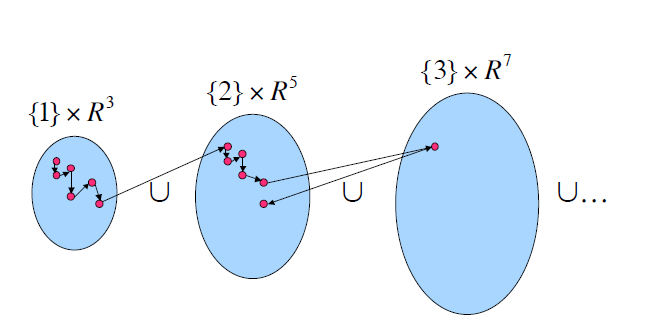
\includegraphics[width=0.5\textwidth]{RJMCMCImage.png}\\ 
Ci limitiamo a considerare i casi in cui, per qualche distribuzione di probabilità di
partenza la probabilità che la catena risieda in un sottoinsieme $A \subset X$ e muova
verso un certo $B\subset X$ sia la stessa qualora si scambino i ruoli di A e di B. Questa
richiesta è detta di equilibrio bilanciato , se verificata da una certa probabilità è una
condizione sufficiente affinchè questa sia stazionaria.


Spesso per attraversare lo spazio X è necessario avere a disposizione diverse tipologie di mosse.
Una tipologia di mossa associa la struttura del modello attuale ad una nuova struttura.
Affinchè la condizione di equilibrio bilanciato sia soddisfatta è necessario che se esiste la mossa $( x \rightarrow x' )$ esista anche la mossa inversa $(x' \rightarrow x)$ .
Si indichi con $j_m (x)$ la probabilità che dallo stato x sia scelta la mossa di tipo m e
si indichi con $j_m^{-1}
(x ) $la probabilità che dallo stato x sia scelta la mossa di tipo m
inversa.
Il problema è che non ha senso paragonare probabilità definite su spazi di dimen-
sione diversa.
Per rendere invisibile alla catena il cambio di dimensionalità basta immergere i due
spazi di dimensione diversa in uno stesso spazio di dimensione maggiore e definire
in tale spazio la probabilità.
Si adotti quindi il seguente protocollo (ideato da Peter Green nel 1995):
\begin{itemize}
\item Si estragga la tipologia di mossa.
\item Si generino r numeri casuali $u\in\mathbb{R}^r$ da una specificata densità g.
\item Si costruisca il nuovo stato attraverso una funzione deterministica h di x e di u.
\begin{equation}
(x' , u' ) = h(x, u)
\end{equation}
In questo caso sono stati indicati con u gli r numeri che sono estratti casualmente
dalla distribuzione g quando si effettua la mossa inversa da x' a x usando la funzione
deterministica inversa
\begin{equation}
(x, u) = h ^{-1}(x' , u ')
\end{equation}
l’equazione di equilibrio bilanciato si può scrivere dunque come
\begin{equation*}
\sum_m \int_{(x,u):(x,x')\in A\times B}j_m(x)\ph(x)g_m(u)\gamma_m(x'|x)dxdu=
\sum_m \int_{(x',u'):(x,x')\in A\times B}j_m^{-1}(x')\ph(x')g_m(u')\gamma_m(x'|x)dx'du'
\end{equation*}
La sommatoria sulle possibili mosse deriva dal fatto che ad ogni iterazione la tipologia di mossa è esclusiva. Una condizione sufficiente non necessaria perchè valga il
bilancio è che esso valga mossa per mossa ovvero
\end{itemize}
\begin{equation*}
 \int_{(x,u):(x,x')\in A\times B}j_m(x)\ph(x)g_m(u)\gamma_m(x'|x)dxdu=
 \int_{(x',u'):(x,x')\in A\times B}j_m^{-1}(x')\ph(x')g_m(u')\gamma_m(x'|x)dx'du'
\end{equation*}
se inoltre la funzione h è un diffeomorfismo vale la formula classica del cambio
di variabili e quindi si può passare dall’uguaglianza integrale all’uguaglianza delle
integrande.
Dal momento che la mossa è fissata si ha che k e k' sono costanti dunque il cambio
di variabili richiesto riguarda solo il vettore dei parametri e delle variabili ausiliarie.
\begin{equation*}
(\theta_k',u')\rightarrow(\theta_k,u)
\end{equation*}
Applicandolo si ottiene
\begin{equation*}
j_m(x)\ph(x)g_m(u)\gamma_m(x'|x)=
j_m^{-1}(x')\ph(x')g_m(u')\gamma_m(x'|x)\left\vert\frac{\partial(\theta_{k'},u') }{\partial(\theta_{k},u) }\right\vert
\end{equation*}
Condizione necessaria affinchè h sia un diffeomorfismo è che
\begin{equation}
dim(\theta_{k'})+dim(u')=dim(\theta_{k})+dim(u)
\end{equation}
detta condizione di \emph{dimension matching} e inoltre deve valere
\begin{equation}
det\left(\frac{\partial(\theta_{k'},u') }{\partial(\theta_{k},u) }\right)\neq 0
\end{equation}
 Si ha dunque in tal caso che
\begin{equation}
\gamma_m(x'|x)=\min\left\lbrace 1,\frac{
j_m^{-1}(x')\ph(x')g_m(u')\gamma_m(x'|x)}
{j_m(x)\ph(x)g_m(u)}
\left\vert\frac{\partial(\theta_{k'},u') }{\partial(\theta_{k},u) }\right\vert 
\right\rbrace
\end{equation}